% !TEX root = main.tex
\documentclass[conference, 10pt]{IEEEtran}
\IEEEoverridecommandlockouts
\usepackage{amsmath,amssymb,amsfonts}
\usepackage{algorithmic}
\usepackage{graphicx}
\usepackage{textcomp}
\usepackage{xcolor}
\usepackage{hyperref} % URLs
\usepackage{bookmark}
\hypersetup{colorlinks=true, linkcolor=black, urlcolor=blue, citecolor=black}
\usepackage[backend=biber,bibencoding=utf8, style=ieee]{biblatex}
\def\BibTeX{{\rm B\kern-.05em{\sc i\kern-.025em b}\kern-.08em
    T\kern-.1667em\lower.7ex\hbox{E}\kern-.125emX}}
\addbibresource{main.bib}

\begin{document}

\title{Benchmarking RabbitMQ: How does horizontal scaling influence
throughput and end-to-end latency across varying cluster sizes?\\
}

\author{\IEEEauthorblockN{Christopher-Julian Müller}
\IEEEauthorblockA{\textit{Technische Universität Berlin} \\
Berlin, Germany \\
christopher-julian.mueller@campus.tu-berlin.de}
}

\maketitle
\begin{abstract}
RabbitMQ is a widely used open-source message broker and its quorum queues use the Raft consensus algorithm to replicate messages across cluster nodes for data safety and high availability. Horizontal scaling is a common strategy to increase message throughput, but it is not obvious whether adding nodes delivers proportional gains when every message must be replicated. Additionally, Raft requires a majority of nodes to acknowledge every write before it is committed, creating a trade-off between fault tolerance and latency that makes it unclear how latency behaves as the cluster grows. We investigate this trade-off by developing a Go CLI benchmark tool and running three experiments, each repeated three times, across cluster sizes of 3, 6 and 9 nodes on Azure infrastructure, measuring maximum throughput with fixed quorum size and end-to-end latency with quorum size equal to the cluster size. Our results show that throughput scales near-linearly (3.11$\times$ at 9 nodes) when quorum size is fixed at 3, while end-to-end mean latency increases from 3.4\,ms to 4.3\,ms and P99 latency rises from 4.6\,ms to 6.0\,ms with growing inter-run variability as more nodes participate in Raft replication. Under heavy load, latency degrades by up to 146$\times$ compared to the ideal baseline. Our results suggest that adding nodes with a fixed quorum size is effective for scaling throughput, but increasing the quorum size carries a significant latency cost that should be weighed carefully against the additional fault tolerance it provides.
\end{abstract}

\section{Introduction}

Most modern software architectures are distributed by design and message brokers play an important role in enabling communication and coordination between different parts of these systems. Using a message broker as an intermediary between components allows services to reliably send messages to each other without needing to know about the details of the recipient's implementation or availability. As a result, message brokers have become a critical component in many distributed systems and their performance can have a significant impact on the overall system's responsiveness and scalability. Among the many available message brokers, RabbitMQ is one of the most widely known and used open-source options. RabbitMQ's Quorum Queues, built on the Raft consensus algorithm~\cite{raft_paper}, are advertised as the go-to queue type for systems that require data safety and high availability but don't rely on time-sensitive messaging (such as stock tickers or instant messaging systems)~\cite{rmq_quorum_docs}.

However, the data safety advantages of Quorum Queues come at a cost. RabbitMQ can be deployed as a cluster of multiple nodes that together form a single logical broker. The Raft consensus algorithm requires every message to be replicated to a majority of these nodes before it is acknowledged, introducing a trade-off: scaling horizontally by adding nodes increases the total capacity and fault tolerance of the cluster, but it also increases the number of nodes that must agree on every write. The resulting overhead from additional network communication, disk writes and internal coordination makes it difficult to predict how throughput and latency will behave as the cluster grows.

As systems scale, understanding how RabbitMQ and its Quorum Queues perform under different load conditions becomes important. Therefore, this work aims to investigate this behavior by focusing on throughput and end-to-end latency as the primary performance metrics across varying cluster sizes and load conditions. By developing and using a custom benchmark CLI tool to benchmark RabbitMQ clusters, we evaluate how these two metrics change under horizontal scaling and identify any diminishing returns that may arise.

The remainder of this paper is structured as follows. Section~II provides background on RabbitMQ, Quorum Queues and the Raft consensus algorithm. Section~III describes the benchmark setup, including the infrastructure, the benchmark tool and the experiments. Section~IV analyzes the measurement results, whereas Section~V outlines directions for future work and Section~VI concludes the paper.
% DONE


\section{Background}

This section introduces the core concepts of RabbitMQ and notable protocols that are relevant to the benchmark experiments presented in this paper. We first describe the AMQP messaging model and how RabbitMQ implements it, then explain how Quorum Queues use the Raft consensus algorithm to provide data safety through replication.

\subsection{RabbitMQ and AMQP}
RabbitMQ is an open-source message broker that implements the Advanced Message Queuing Protocol (AMQP)~\cite{amqp_spec}, \cite{rmq_amqp_docs}. In AMQP, publishers send messages to an \textit{exchange}, which routes them to one or more \textit{queues} based on configurable \textit{bindings} and routing keys. Consumers then read messages from queues. This indirection decouples producers from consumers where neither side needs to be aware of the other and messages can be buffered in queues when consumers are temporarily unavailable~\cite{Magnoni_2015}.

A RabbitMQ cluster consists of multiple nodes that share metadata about exchanges, queues and bindings. Clients can connect to any node in the cluster. When a client publishes to or consumes from a queue whose data resides on a different node, the receiving node proxies the operation to the node that owns the queue~\cite{rmq_clustering_docs}. This proxy path adds an extra network hop compared to connecting directly to the queue leader node.

\subsection{Quorum Queues and Raft}
Classic Mirrored Queues were RabbitMQ's former queue type for queue replication across cluster nodes. However, they had significant shortcomings regarding data consistency: the replication algorithm could produce message loss and administrators were forced to choose between availability and data safety during network partitions~\cite{rmq_ha_upgrade_blog}. Quorum Queues were introduced as a replacement and are now the recommended queue type for workloads that require data safety and high availability.

Under the Raft consensus algorithm~\cite{raft_paper}, each quorum queue is implemented as a replicated state machine with one replica on each cluster node, where one serves as the \textit{leader} and the rest as \textit{followers}. The leader handles all reads and writes for the queue. When a publisher sends a message, the leader appends it to its local write-ahead log (WAL) and replicates the entry to all followers. The message is only considered committed once a \textit{majority} of members (the quorum) have persisted the entry. The leader only acknowledges the message back to the publisher once the commit is complete.

The quorum for a cluster of size $n$ is $\lfloor n/2 \rfloor + 1$. This means a three-node cluster tolerates one node failure (quorum of two), a five-node cluster tolerates two (quorum of three) and so on. While adding nodes increases fault tolerance, it also increases the number of acknowledgements required before a message is committed. Each additional member that must persist a log entry adds further disk I/O and network round trips to the commit path, which reduces overall queue throughput as the cluster grows~\cite{rmq_quorum_docs}. The effect of this replication overhead on throughput and end-to-end latency as the cluster grows is the central question of this work. Figure~\ref{fig:raft_replication} illustrates the replication process for a six-node quorum queue.

\begin{figure}[!ht]
\centering
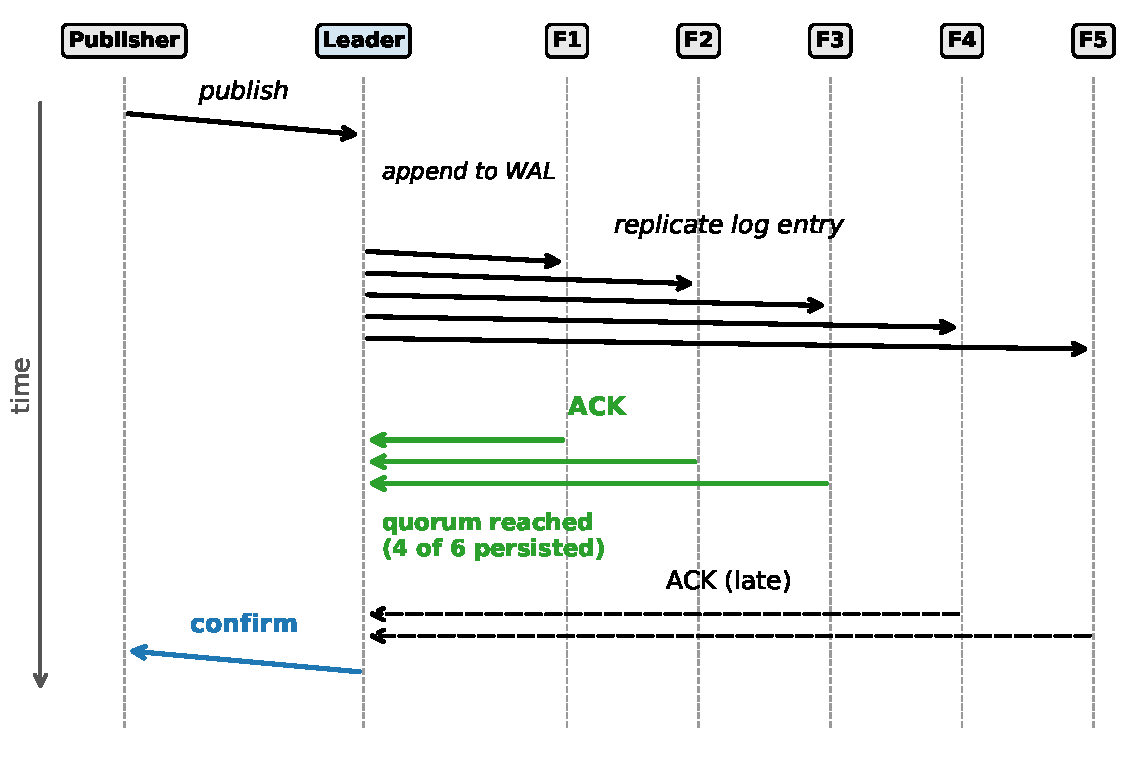
\includegraphics[width=1.04\columnwidth]{../results/plots/0A_raft_replication.pdf}
\caption{Raft replication sequence for a 6-node quorum queue. The leader appends the message to its WAL, replicates to all followers and confirms to the publisher once a quorum (4 of 6) has persisted the entry.}
\label{fig:raft_replication}
\end{figure}

\subsection{Publisher Confirms}
By default, AMQP publishers receive no feedback on whether a message was successfully enqueued. RabbitMQ's publisher confirms extension addresses this by having the broker acknowledge each message after it has been committed~\cite{rmq_confirms_docs}. For quorum queues, this means the confirm is only sent after the Raft commit, making confirms a signal that the message has been replicated to a majority of nodes.

Publisher confirms can operate in two modes. In \textit{synchronous} mode, the publisher waits for each confirm before sending the next message. This serializes publishes and measures the round-trip latency of the Raft replication. In \textit{asynchronous} mode, the publisher sends messages continuously and processes confirms as they arrive, allowing multiple messages to be in flight simultaneously. This pipelined approach achieves higher throughput at the cost of more complex flow control. Both modes are used in our benchmark experiments to benchmark cluster performance under different scenarios.

\section{Experimental Setup}

\subsection{Infrastructure}
All experiments were done on Microsoft Azure using virtual machines provisioned via Terraform. The RabbitMQ cluster nodes run on \texttt{Standard\_D4s\_v6} instances (4 vCPUs, 16\,GB RAM) running Ubuntu 24.04 LTS. Besides a 30\,GB Premium SSD as OS disk, each cluster node has a additional 256\,GB Premium SSD v2 (NVMe) disk configured with 10{,}000 IOPS and 600\,MB/s read/write, mounted at the RabbitMQ data directory. The reason for using additional Premium SSD v2 disks is that we can't use them as OS disks, whereas Standard and Premium SSDs below 1\,TB in size use bursting, where I/O performance fluctuates depending on accumulated burst credits. This would pollute benchmark results. On the other hand, provisioning a 1\,TB or larger non-bursting OS disk for every cluster node would be too costly. Premium SSD v2 disks avoid this problem by providing consistent, non-bursting performance at a lower cost.

The load generator runs on a \texttt{Standard\_F32s\_v2} instance (32 vCPUs, 64\,GB RAM). By overprovisioning the load generator's resources, we ensure it does not become a bottleneck itself. All virtual machines are deployed within the same Azure Virtual Network and subnet, so that AMQP traffic between the load generator and the cluster nodes traverses only the internal network, which again removes external interference to our benchmark results.

Cluster formation is automated through a cloud-init script that installs RabbitMQ 4.2.2 and its Erlang runtime, mounts the NVMe data disk and joins each node to a shared cluster using a common Erlang cookie. We benchmarked cluster sizes of 3, 6 and 9 nodes. For each cluster size, the same Terraform configuration was re-applied with only the node count changed, keeping all other parameters the same. Figure~\ref{fig:infrastructure} shows an overview of the infrastructure setup.

\begin{figure}[h]
\centering
\includegraphics[width=\columnwidth]{../results/plots/0C_infrastructure.pdf}
\caption{Infrastructure setup. The load generator connects to all cluster nodes over the internal Azure Virtual Network via AMQP.}
\label{fig:infrastructure}
\end{figure}

\subsection{Benchmark Tool}
We developed a Go CLI tool to execute the benchmark experiments. The tool connects to the RabbitMQ cluster, creates the quorum queues, runs the specified experiment with the given CLI parameters and records per-second metrics to CSV files alongside a JSON configuration file that contains all entered CLI parameters for traceability.

\subsubsection{Latency Measurement}
Latency is measured end-to-end by embedding a nanosecond-precision timestamp in each message header at publish time. The consumer extracts this timestamp upon delivery and computes the difference to obtain the end-to-end latency, covering the full path from publisher to consumer including Raft replication.

\subsubsection{Throughput Measurement}
Throughput is derived from publisher confirmations. Each confirmed message increments the throughput counter for the current one-second recording window. This ensures that only messages that have been committed by the Raft quorum are counted.

\subsubsection{Recording and Histograms}
Our benchmark CLI uses two HDR histograms to capture latency distributions. A \textit{window histogram} is reset every second and written to the results CSV, providing a time series of latency percentiles throughout the experiment. A \textit{global histogram} accumulates all measurements from the end of the warmup period onward and is used to compute the final summary statistics such as the P99 latency. To avoid per-message mutex contention at high message rates, latency values are submitted in batches of 100 through a buffered channel to a separate recording goroutine.

The benchmark CLI supports a configurable warmup phase during which measurements are excluded from the recorded results. In our experiments, we did not use the warmup parameter and instead filtered out rows during the analysis stage.

\subsection{Experimental Design}

We implemented three experiments to examine different aspects of how horizontal scaling affects RabbitMQ throughput and latency. Table~\ref{tab:parameters} lists the CLI parameters used for each experiment.

\begin{table}[t]
\centering
\caption{Benchmark parameters used for each experiment.}
\label{tab:parameters}
\footnotesize
\setlength{\tabcolsep}{6pt}
\begin{tabular}{@{}l c c c@{}}
\textbf{Parameter} & \textbf{Linear Capacity} & \textbf{Ideal Latency} & \textbf{Stress Latency} \\
\hline
Duration (s)          & 3{,}600  & 3{,}600  & 3{,}600 \\
Msg.\ size (bytes)    & 1{,}024  & 1{,}024  & 1{,}024 \\
Publishers            & 160/node & 1        & 10/node + 1 \\
Consumers             & 0        & 1        & 0 \\
Queues/node           & 4        & 1        & 4 \\
Quorum size           & 3 (fixed) & = cluster size & = cluster size \\
Queue max length      & 1{,}000  & ---       & 1{,}000 \\
Overflow              & drop-head & ---      & drop-head \\
\hline
\end{tabular}
\end{table}

\subsubsection{Linear Capacity}
The linear-capacity experiment measures the maximum throughput of the cluster. Multiple quorum queues are created per node and publishers are distributed evenly across all nodes, each with their own AMQP connection to avoid sharing bottlenecks. Publishers use asynchronous confirms with a pipeline depth of up to 2{,}000 messages in flight, allowing the publish rate to be decoupled from confirmation processing.

Since this experiment focuses purely on throughput, we run it without consumers. However, without consumers, messages accumulate in memory on the cluster nodes before they get written to disk. When a node's memory usage exceeds its configured threshold (60\% of RAM by default), RabbitMQ raises a memory alarm and blocks all publishing connections on that node until memory drops below the threshold again~\cite{rmq_memory_docs, rmq_flow_control_docs}. Keeping up with the publish rate through consumers would require a large number of them, which would add significant load to the cluster nodes and take away resources that we want to dedicate entirely to publishers. Instead, we configure each queue with a maximum length and a drop-head overflow strategy, which causes the broker to discard the oldest messages when the queue is full. This keeps memory usage bounded without requiring consumers, allowing us to use all available node resources for maximizing throughput.

As the cluster grows, both the total number of queues and publishers scale proportionally since the queue and publisher parameters in this experiment are per node, so that each node receives a comparable amount of load.

\subsubsection{Ideal Latency}
To isolate the latency floor of the Raft consensus under minimal contention within this experiment, a single quorum queue is created and both the publisher and consumer connect directly to the queue's leader node. The publisher operates in synchronous confirm mode, waiting for each message to be committed by the quorum before sending the next one. This ensures that each latency sample captures exactly one Raft replication round trip without interference from concurrent messages. The resulting measurements represent the best-case latency for a given cluster size.

\subsubsection{Stress Latency}
The stress-latency experiment measures how latency degrades when the cluster is under heavy load. It combines the measurement setup of the ideal-latency experiment with background stress traffic similar to the linear-capacity experiment. A single publisher and consumer pair connects to the queue leader and records end-to-end latency using synchronous confirms, while a configurable number of stress publishers flood separate queues across all nodes using asynchronous confirms. The stress traffic competes for CPU, disk I/O and Raft coordination resources without polluting the latency measurements, since the measured and stress traffic use separate queues and connections.

\subsubsection{Quorum Size Strategy}

The experiments use two different quorum size configurations depending on what aspect of horizontal scaling they measure. The linear-capacity experiment fixes the quorum size at 3 (RabbitMQ default) regardless of cluster size. RabbitMQ recommends keeping quorum queues small, as throughput decreases with more members and advises against exceeding 7 members~\cite{rmq_quorum_docs}. In practice, cluster nodes are therefore added to host more small independent quorum groups rather than to increase the quorum size of existing queues. Since both queues and publishers scale per node, the linear-capacity experiment measures whether aggregate throughput increases proportionally with cluster size.

The ideal-latency and stress-latency experiments take the opposite approach and set the quorum size equal to the cluster size (3, 6 or 9). Since both experiments measure a single queue, a fixed quorum size of 3 would leave the additional nodes as passive observers that do not participate in Raft consensus for that queue and would likely produce similar results across all cluster sizes. By making every node a quorum member, our latency measurements capture the coordination cost of the whole cluster rather than just a 3-node subset of it.
\section{Results}
This section analyzes the measurements collected across three experiments and three cluster sizes (3, 6 and 9 nodes), where each experiment was repeated three times with a one hour duration. For configuration and parameter details that were used to achieve these measurements, see Section~III.

\subsection{Throughput}
Table~\ref{tab:throughput} summarizes the throughput results from the linear-capacity experiment. Each node was loaded with 160 publishers using asynchronous confirms, resulting in 480, 960 and 1{,}440 total publishers for the 3, 6 and 9-node clusters respectively.

\begin{table}[h]
\centering
\caption{Summary of throughput results from the linear-capacity experiment.}
\label{tab:throughput}
\begin{tabular}{l r r r}
\hline
\textbf{Cluster} & \textbf{Mean (msgs/s)} & \textbf{Scaling Factor} & \textbf{Std Dev} \\
\hline
3 Nodes  & 98{,}134  & 1.00$\times$ & 508  \\
6 Nodes  & 210{,}785 & 2.15$\times$ & 3{,}433 \\
9 Nodes  & 304{,}867 & 3.11$\times$ & 2{,}646 \\
\hline
\end{tabular}
\end{table}

The cluster achieves approximately linear throughput scaling. Tripling the node count from 3 to 9 yields a 3.11$\times$ improvement, which is consistent with the 3$\times$ increase in cluster nodes. Since the quorum size is fixed at 3, adding nodes introduces new queues and publishers without increasing per-message replication overhead. Only three replicas must acknowledge each write regardless of cluster size, so the additional nodes contribute more publishing capacity without adding consensus overhead.

Per-node throughput remains consistent across all cluster configurations, ranging from approximately 32{,}700 msgs/s per node (3-node) to 35{,}100 msgs/s per node (6-node) and 33{,}900 msgs/s per node (9-node). Since the number of queues and publishers scales proportionally with the node count, each node handles the same workload regardless of cluster size. As a result, we see a relatively consistent per-node throughput with a low inter-run standard deviation of 508--3{,}433 msgs/s. As seen in Figure~\ref{fig:throughput_ts}, the throughput is stable across the one-hour benchmark duration.

\begin{figure}[h]
\centering
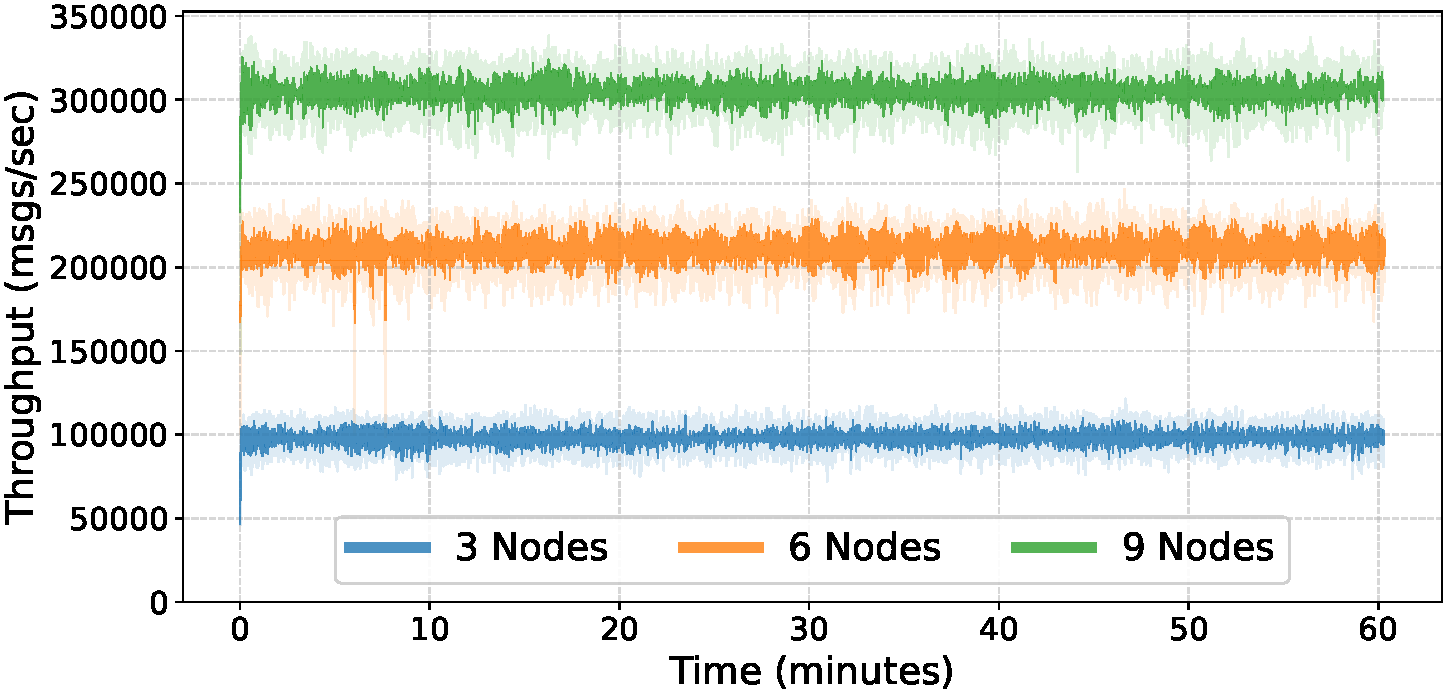
\includegraphics[width=\columnwidth]{../results/plots/6_throughput_timeseries.pdf}
\caption{Per-second throughput averaged across all three runs for each cluster size, with shaded bands showing inter-run standard deviation.}
\label{fig:throughput_ts}
\end{figure}

Figure~\ref{fig:throughput} shows the expected throughput if performance scaled linearly from the 3-node result. The error bars represent inter-run standard deviation across all our three benchmark runs. The measured values are close to the expected line, with the 6-node and 9-node clusters slightly exceeding it.

\begin{figure}[h]
\centering
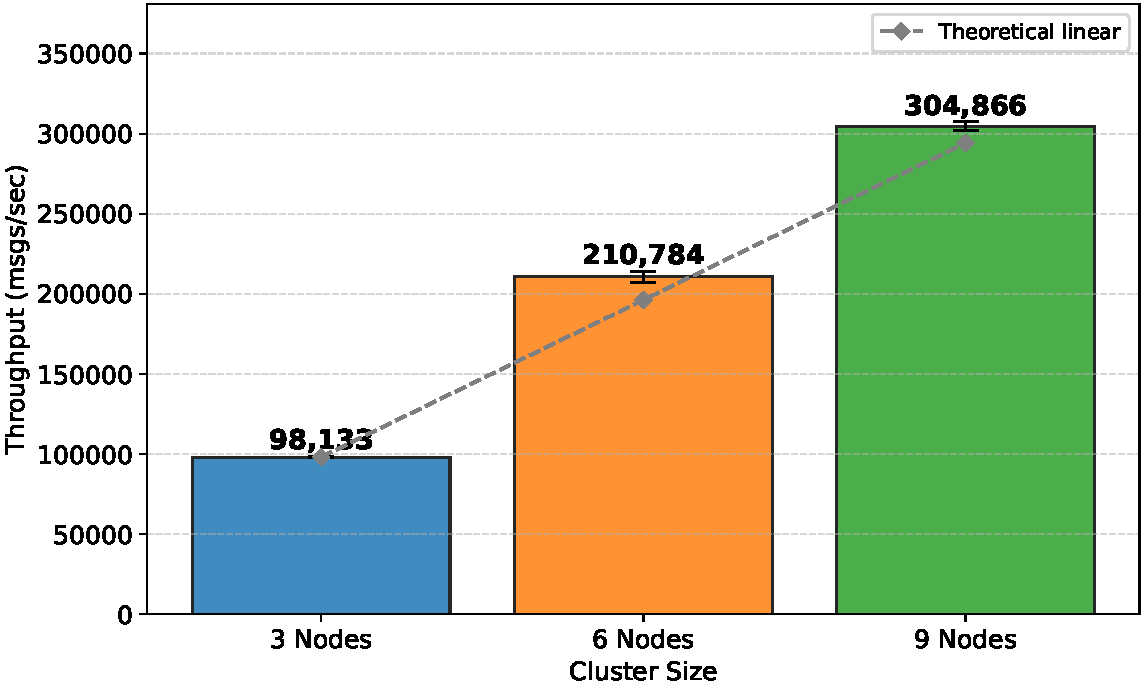
\includegraphics[width=\columnwidth]{../results/plots/1_throughput_scalability.pdf}
\caption{Mean throughput per cluster size with inter-run standard deviation error bars.}
\label{fig:throughput}
\end{figure}

\subsection{Latency Under Ideal Conditions}
\label{subsec:ideal_latency_results}
The ideal-latency experiment isolates the Raft consensus latency by using a single publisher and consumer connected directly to the queue leader node. Table~\ref{tab:ideal_latency} summarizes the results. Unlike the throughput experiment, the quorum size equals the cluster size here, so every node participates in consensus.

\begin{table}[h]
\centering
\caption{Summary of results from the ideal-latency experiment.}
\label{tab:ideal_latency}
\begin{tabular}{l c r}
\hline
\textbf{Cluster} & \textbf{Mean ($\mu$s)} & \textbf{P99 ($\mu$s)} \\
\hline
3 Nodes & 3{,}420 & 4{,}550 \\
6 Nodes & 4{,}000 & 4{,}690 \\
9 Nodes & 4{,}290 & 5{,}950 \\
\hline
\end{tabular}
\end{table}

Mean latency increases with cluster size: +17\% from 3 to 6 nodes and +7\% from 6 to 9 nodes. This slower increase is consistent with Raft's majority-based commit rule. A message is committed once a majority of members have persisted it and the commit latency is determined by the speed of the fastest majority rather than the slowest node~\cite{raft_paper}. Going from 3 to 6 nodes raises the required quorum from 2 to 4, a significant jump. Going from 6 to 9 nodes raises it from 4 to 5, a smaller relative increase that results in a smaller latency impact.

Figure~\ref{fig:consensus_tax} shows mean and P99 latency for each cluster size, with shaded bands representing inter-run standard deviation across all our three benchmark runs. While the mean latency bands remain narrow across all sizes, the P99 band grows noticeably wider for the 9-node cluster. The P99 latency increases by only 3\% from 3 to 6 nodes but jumps by 27\% from 6 to 9 nodes. With a quorum of 5 out of 9, the leader must wait for 5 disk fsyncs (flushes that ensure data is written to disk) across the cluster. With 9 nodes, the chance that at least one follower is temporarily slow increases, which pushes more requests into the P99 range.

\begin{figure}[h]
\centering
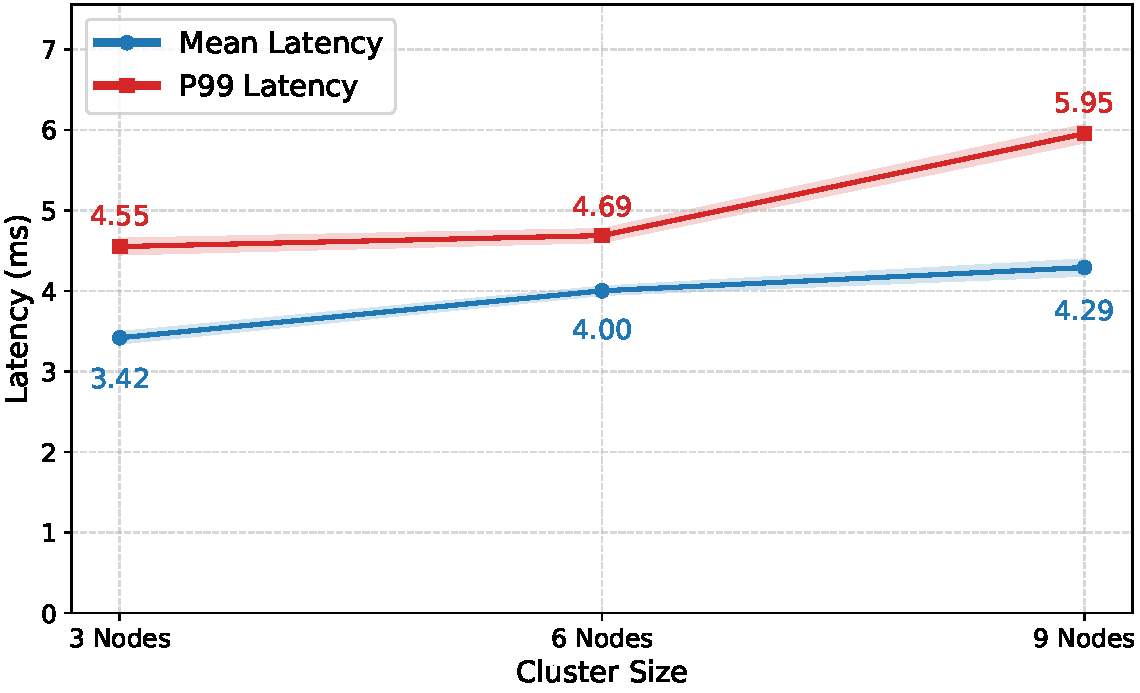
\includegraphics[width=\columnwidth]{../results/plots/3_consensus_tax.pdf}
\caption{Mean and P99 latency across cluster sizes. Shaded bands show inter-run standard deviation.}
\label{fig:consensus_tax}
\end{figure}

\subsection{Latency Under Load}
\label{subsec:latency_under_load}
The stress-latency experiment measures how latency degrades when the cluster is under heavy background load. A single publisher with synchronous confirms measures the latency while stress publishers flood the cluster using asynchronous confirms. Table~\ref{tab:stress_latency} summarizes the results.

\begin{table}[h]
\centering
\caption{Summary of results from the stress-latency experiment. Coverage shows the percentage of seconds in which at least one latency sample was recorded.}
\label{tab:stress_latency}
\begin{tabular}{l c c r}
\hline
\textbf{Cluster} & \textbf{Mean (ms)} & \textbf{P99 vs.\ Ideal P99} & \textbf{Coverage} \\
\hline
3 Nodes & 140.6 & 61$\times$  & 6.80\% (245/3607) \\
6 Nodes & 388.2 & 128$\times$ & 2.60\% (94/3608)  \\
9 Nodes & 611.9 & 146$\times$ & 1.64\% (59/3604)  \\
\hline
\end{tabular}
\end{table}

Latency under load is 61$\times$ to 146$\times$ worse than the ideal baseline (see Section~\ref{subsec:ideal_latency_results}). The low measurement coverage is not a measurement issue but a consequence of the experimental design. With synchronous confirms at 140--612\,ms per message, the measured publisher can only send approximately 2--7 messages per second. Since each CSV row aggregates a batch of 100 latency samples, filling one row takes 14--62 seconds, which matches the observed coverage ratios. The low inter-run standard deviation of the P99 values (5--27\,ms) shows that the system reaches a consistently degraded state across repeated runs rather than fluctuating unpredictably.

The large latency increase is likely caused by Erlang scheduler contention as CPU, disk and network all remain well below capacity (see Section~\ref{subsec:resource_utilization}). The stress publishers create heavy load across all nodes, including the node that hosts the measured queue's leader. Each quorum queue replica is limited to a single CPU core~\cite{rmq_queues_docs}, so the stress queue processes on the leader node compete with the measured queue's process for Erlang scheduler time. Although the stress publishers target separate queues, they slow down the measured queue's Raft process by consuming scheduler capacity on the same node. The RabbitMQ flow control mechanism further throttles publishers when internal buffers fill up~\cite{rmq_flow_control_docs}, adding to the latency increase.

Additionally, latency roughly quadruples from 3 to 9 nodes, growing faster than the cluster size itself. This is partly due to the quorum size increasing with the cluster size (from 3 to 9), which means more nodes must acknowledge each write under contention. However, the number of stress publishers also grows with the cluster size (10 per node, so 30 to 90 total), which means that the increased background load and the larger quorum both contribute to the latency degradation. Our experiment does not isolate these two factors, so the observed increase reflects the combined effect of more replication overhead and more resource contention. The stress-latency results demonstrate that when both quorum size and load grow with node count, latency degrades more than proportionally.

\begin{figure}[h]
\centering
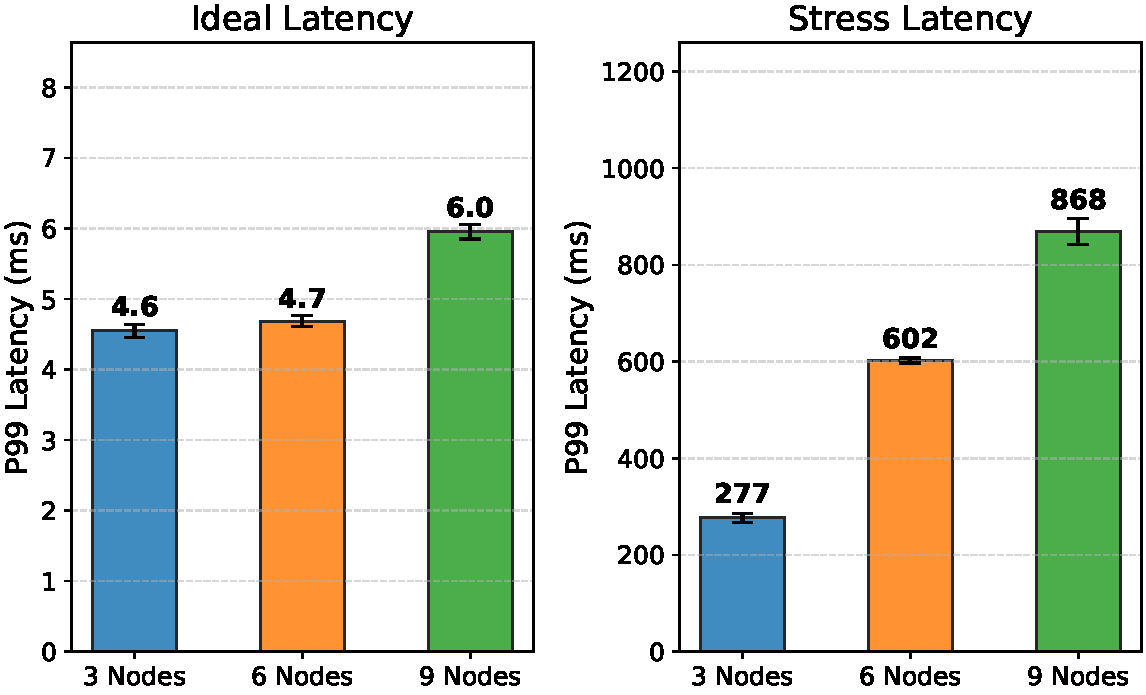
\includegraphics[width=\columnwidth]{../results/plots/2_latency_gradient.pdf}
\caption{Comparison of ideal (left) vs. stress (right) P99 latency. Note the different y-axis scales and error bars showing inter-run standard deviation.}
\label{fig:latency_gradient}
\end{figure}
\newpage

Figure~\ref{fig:latency_gradient} shows the contrast between ideal and stress P99 latency. The left panel shows ideal latency in the single-digit millisecond range while the right panel shows stress latency reaching hundreds of milliseconds.

\subsection{Resource Utilization}
\label{subsec:resource_utilization}
Figure~\ref{fig:resources} shows the cluster-wide average CPU utilization and total disk write throughput during the 9-node linear-capacity run, collected from Azure Monitor metrics. CPU averages around 60--65\% across the nine nodes throughout the benchmark. The total disk write throughput across all nodes is approximately 1{,}200\,MB/s, which corresponds to roughly 133\,MB/s per node and thus well below the 600\,MB/s provisioned per disk. Both metrics remain stable and demonstrate that the consistent throughput observed in Section~IV-A is matched by consistent resource consumption.

Network bandwidth is also not a limiting factor. Each D4s\_v6 node supports up to 12.5\,Gbps of network throughput and Azure Virtual Networks have no additional bandwidth limit. At the observed 9-node throughput of approximately 305{,}000 msgs/s with 1\,KB messages and a quorum size of 3, the total replication traffic is roughly 900\,MB/s across the cluster, or about 100\,MB/s per node, which is approximately 6\% of the per-node network capacity.

Neither CPU, disk I/O nor network are close to saturation, yet the per-node throughput peaks at approximately 34{,}000 msgs/s even after adding more publishers during the experiment. This suggests that the bottleneck lies within RabbitMQ's software architecture rather than the underlying hardware. As discussed in Section~\ref{subsec:latency_under_load}, each quorum queue replica is limited to a single CPU core. With four queues per node, only four leader processes handle the entire publishing load, which likely imposes the throughput ceiling before hardware resources are exhausted.

\begin{figure}[h]
\centering
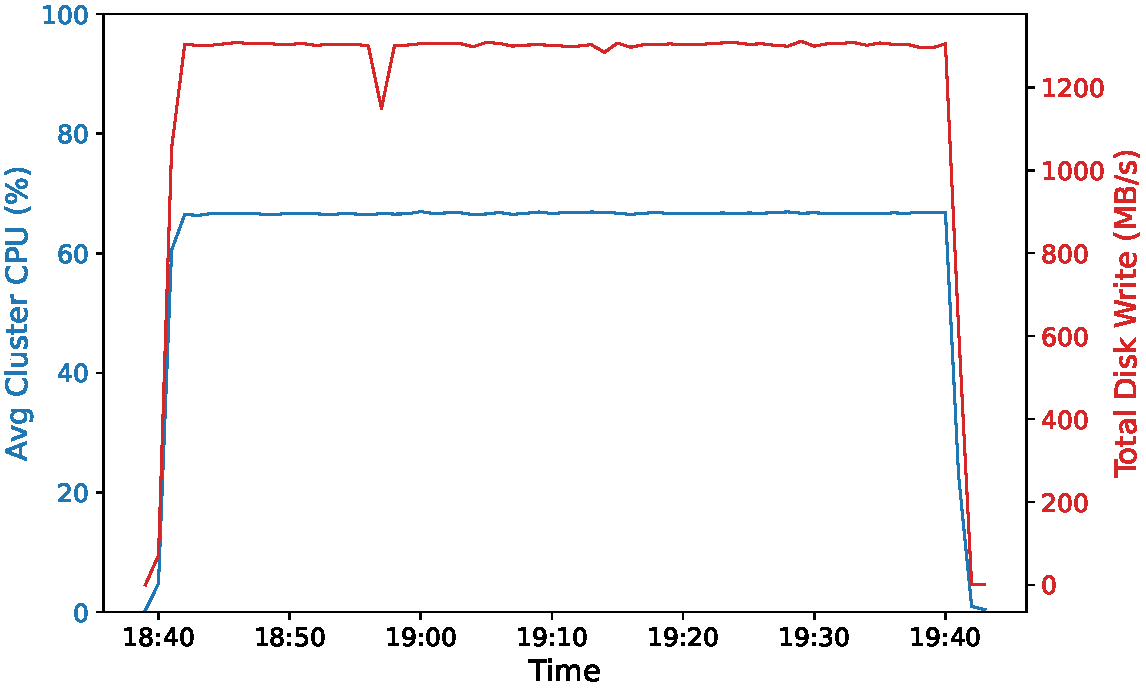
\includegraphics[width=\columnwidth]{../results/plots/4_resource_saturation.pdf}
\caption{Cluster-wide CPU utilization and disk write throughput during a single 9-node linear-capacity run.}
\label{fig:resources}
\end{figure}
\section{Future Work}

Our experiments focus mainly on the theoretical capabilities of scaling quorum queues horizontally under controlled conditions. In the future, it seems promising to shift the focus towards scenarios that are closer to production environments:

\textbf{Throughput experiment with consumers.} Our linear-capacity experiment measures publish throughput without consumers, using the drop-head overflow strategy to bound memory usage. In a production system, consumers must keep up with the publish rate. Adding consumers introduces additional load on the same single Erlang process that already serializes publishes, which must then also track delivery state, process acknowledgements and manage queue compaction. Measuring throughput with active consumers would provide a more realistic picture of sustainable cluster capacity.

\textbf{Throughput bottleneck} The resource utilization analysis in Section~IV shows that CPU, disk and network are all well below saturation, yet per-node throughput peaks at approximately 34{,}000 msgs/s. It would be interesting to dive deeper into RabbitMQ internals to pinpoint the component that bottlenecks the throughput in our setup.

\textbf{Message variation.} All experiments use a fixed message size of 1\,KB. Message size affects per-message disk overhead, network bandwidth consumption and internal batching efficiency. Smaller messages (e.g. 64 bytes, typical for routing or command payloads) would increase the per-message overhead relative to payload size, while larger messages (e.g. 64\,KB) would shift the bottleneck toward disk and network throughput. Testing across a range of message sizes would reveal whether the observed scaling results hold or change under different payload sizes and characteristics.

\textbf{Fault tolerance under load.} Quorum queues exist primarily to provide data safety during node failures, yet none of our experiments include a failure scenario. Measuring how throughput and latency behave when a node is killed during a benchmark and how quickly the cluster recovers would reveal how different cluster sizes handle failures in practice. In the throughput experiment with quorum size 3, a node failure only affects the queues that had a replica on that node, while the remaining queues continue operating uninterrupted. In the latency experiments with quorum size equal to the cluster size, every node is a voting member and the impact would be more immediate.

\section{Conclusion}

This paper investigated how horizontal scaling influences throughput and end-to-end latency of RabbitMQ quorum queues across cluster sizes of 3, 6 and 9 nodes. We developed a Go CLI benchmark tool that measures both metrics using publisher confirms and nanosecond-precision timestamps and ran three experiments over one-hour measurement windows on Microsoft Azure infrastructure.

The results show that the answer depends on how the cluster is scaled. When quorum size is fixed at 3 and nodes are added to host additional independent quorum groups, throughput scales near-linearly. Tripling the cluster from 3 to 9 nodes yielded a 3.16$\times$ throughput increase with stable per-node throughput around 34{,}000 msgs/s. This shows that RabbitMQ can effectively distribute load across nodes when the quorum size remains constant.

However, when quorum size grows with the cluster, latency increases noticeably. The end-to-end latency floor rose from 3.5\,ms (3 nodes) to 4.2\,ms (9 nodes) in mean and from 4.6\,ms to 5.9\,ms at P99. Notably, the P99 variability also increased: the P99 standard deviation grew from 330\,$\mu$s to 1{,}464\,$\mu$s as more nodes participated in Raft replication. Under heavy load, latency degraded by 42$\times$ to 146$\times$ compared to the ideal baseline, with the 9-node cluster reaching a mean latency above 600\,ms. These results highlight that increasing the quorum size beyond 3 carries a significant and growing latency cost, especially under contention.

We also showed that the throughput ceiling is not caused by hardware limitations. CPU, disk and network utilization all remained well below their provisioned capacity during the 9-node throughput experiment. This points to RabbitMQ's internal architecture as the limiting factor, likely the single Erlang process that serializes Raft log entries per quorum queue.

In summary, horizontal scaling of RabbitMQ is effective for increasing aggregate throughput when quorum size stays fixed, but increasing quorum size with the cluster leads to growing latency costs. Based on our measurements, a quorum size of 3 is effective for throughput-sensitive workloads. However, our experiments only tested quorum sizes of 3, 6 and 9. Intermediate sizes such as 5 or 7, which RabbitMQ documentation lists as recommended upper bounds~\cite{rmq_quorum_docs}, may offer a different trade-off between fault tolerance and latency that remains to be evaluated.

\newpage
\printbibliography
\end{document}
